\section{Experiments}

\subsection{Simulated experiments}

A task in a simulated environment was learned first to see whether a NAF neural
network could learn to move the end-effector to arbitrarily set goal positions.
The same layout of the network was used as described in section
\ref{sec:distributed_naf}. All poses were 2-dimensional where end-effector and
goal pose was concatenated as input to the network. Rewards were set to $-2$
where the arm ends up outside of the working space, for other all other
successor states the rewards were set to $\exp\left(-1000|\mathbf{x}_e -
\mathbf{x}_g|^2\right) - 1$ where $\mathbf{x}_e$ is the end-effector pose and
$\mathbf{x}_g$ is the goal pose. This makes the reward equal to $0$ close to
the goal and rapidly decay to $-1$ further from the goal. Discount factor was
set to $0.98$ and the Adam optimizer was used with learning rate $0.0001$ on a
batch size of $512$.

The replay buffer was sampled from like described in section
\ref{sec:prio_sampling} with $\alpha = 1$ and $\beta$ in iteration $i$ out of a
total amount of iterations $i_{tot}$ was set according to:

\begin{equation}
    \beta_i = \exp \left( 10(i - i_{tot}) / i_{tot}\right)
\end{equation}

For sampling, a binary tree was used where the value of a parent equals the
sum of its children \cite{schaul2015prioritized}. This way, sampling one
sample from a total of $N$ samples is $\mathcal{O}(\log_2(N))$. The loss
was defined as the mean square error of the sum of temporal-difference
errors.

\begin{figure}[h]
    \centering
    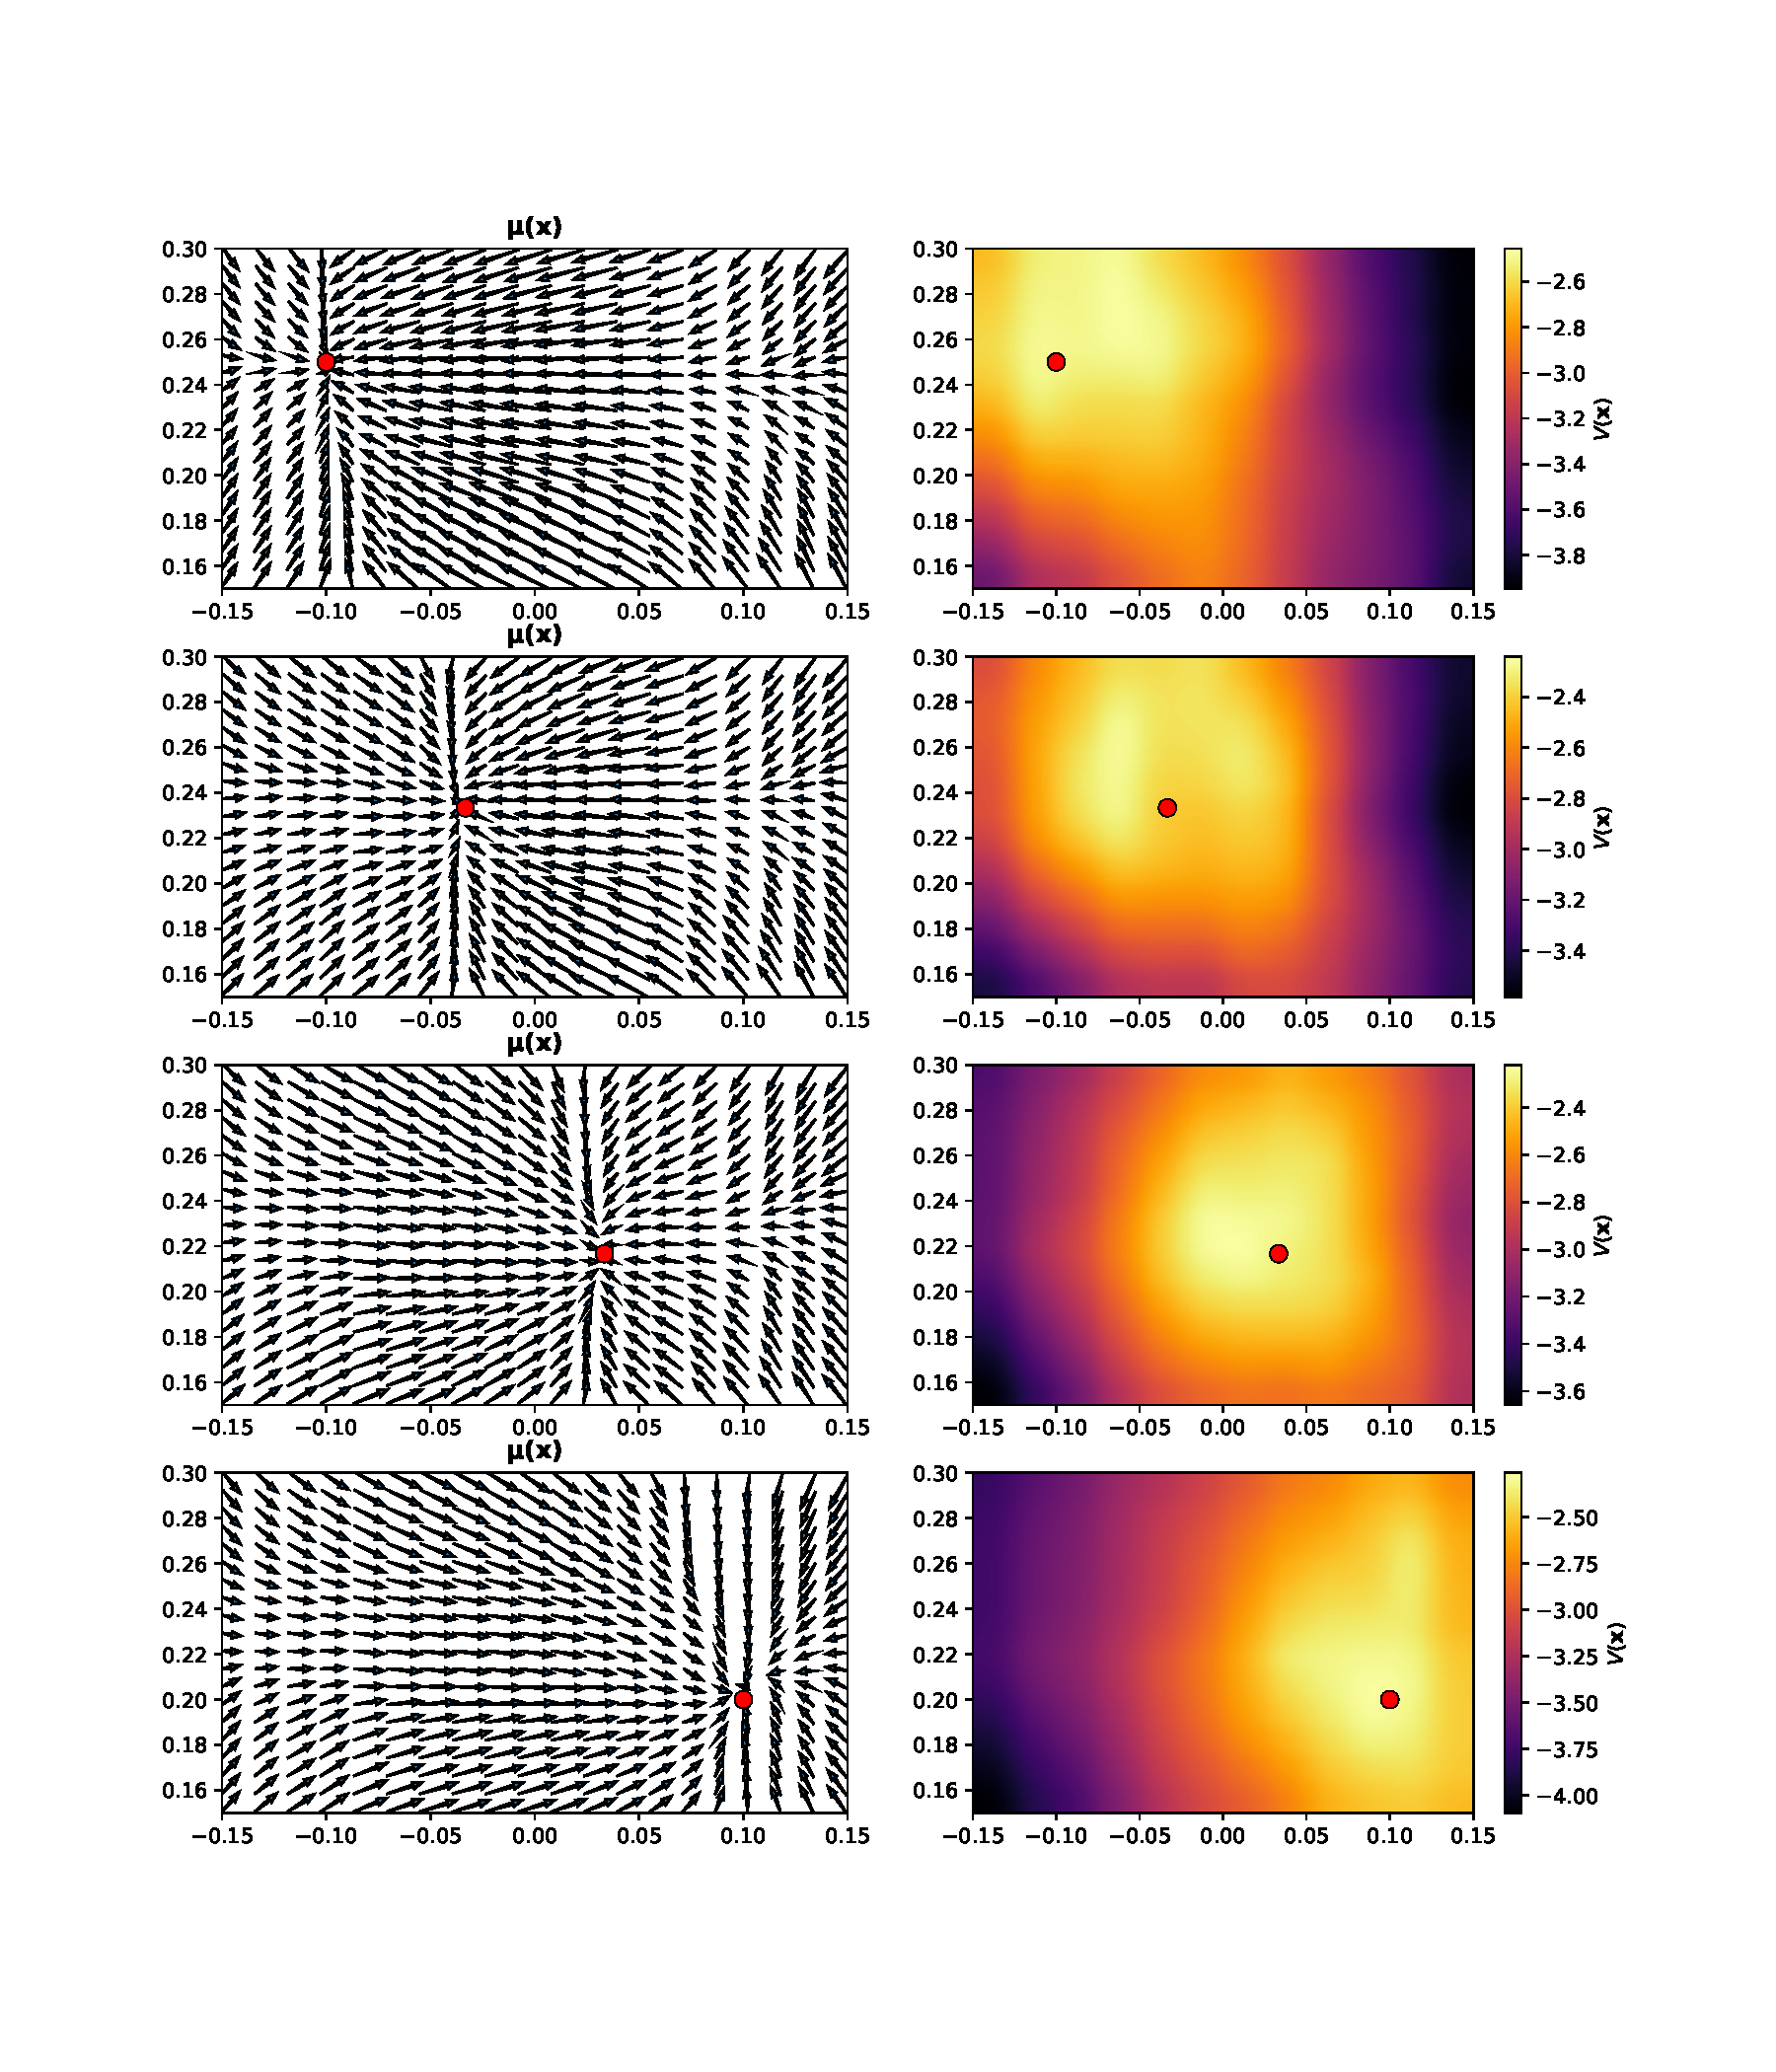
\includegraphics[width=\textwidth]{res/moving_goal_summary.pdf}

    \caption{Trained policy and value function for randomly set goals.
    Vertical and horizontal axes are end-effector positions. Red dot is goal
    position. Left figure shows the learned policy, right side shows the
    learned value function.}
    
\end{figure}
